\documentclass[12pt,a4paper]{article}
\usepackage[utf8]{inputenc}
\usepackage[spanish,es-tabla]{babel}
\usepackage{geometry}
\usepackage{graphicx}
\usepackage{multirow}
\usepackage{tabularx}
\usepackage{mathptmx}
\usepackage{fancyhdr}
\usepackage{array}
\usepackage[table]{xcolor}
\usepackage{titlesec}
\usepackage{setspace}
\usepackage{microtype}
\usepackage{lastpage}
\usepackage{booktabs}
\usepackage{enumitem}
\usepackage{amsmath}
\usepackage{amsfonts}
\usepackage{amssymb}

\graphicspath{{images/}{../images/}{./}}

\geometry{
    top=4.7cm,
    bottom=2.5cm,
    left=2.5cm,
    right=2.5cm,
    headheight=3.9cm,
    headsep=0.4cm
}

\setstretch{1.15}
\setlength{\parindent}{0pt}
\setlength{\parskip}{0.45em}
\setlength{\tabcolsep}{4pt}

\titleformat{\section}
  {\normalfont\fontsize{12}{14.5}\bfseries}{\thesection.}{0.6em}{\uppercase}
\titlespacing*{\section}
  {0pt}{1.8ex plus 0.4ex minus 0.2ex}{0.6ex plus 0.2ex}

\titleformat{\subsection}
  {\normalfont\fontsize{11.5}{13.5}\bfseries}{\thesubsection.}{0.5em}{}
\titlespacing*{\subsection}
  {0pt}{1.4ex plus 0.3ex minus 0.1ex}{0.4ex plus 0.1ex}

\titleformat{\subsubsection}
  {\normalfont\fontsize{10.5}{12.5}\bfseries\itshape}{\thesubsubsection.}{0.4em}{}
\titlespacing*{\subsubsection}
  {0pt}{1.1ex plus 0.2ex minus 0.1ex}{0.3ex plus 0.1ex}

\newcolumntype{Y}{>{\centering\arraybackslash}X}
\newcolumntype{L}{>{\raggedright\arraybackslash}X}
\newcolumntype{C}{>{\centering\arraybackslash}X}

\definecolor{headerred}{RGB}{180, 0, 0}
\definecolor{darkred}{RGB}{140, 0, 0}
\definecolor{lightgraybg}{RGB}{248, 248, 248}
\definecolor{tableheader}{RGB}{232, 238, 246}

\newcommand{\docCodigo}{TI-SIGE-ENT-S1-007}
\newcommand{\docVersion}{1.0}
\newcommand{\docProceso}{CIERRE DE FASE / CONSOLIDACIÓN SEMANA 1}
\newcommand{\docElaboracion}{24/08/2026}
\newcommand{\docRevision}{PENDIENTE DE REVISIÓN}
\newcommand{\docTitulo}{ENTREGABLE GENERAL Y CONSOLIDADO DE LA SEMANA 1}
\newcommand{\docOrganizacion}{FACULTAD DE INGENIERÍA EN SISTEMAS, ELECTRÓNICA E INDUSTRIAL}
\newcommand{\docSubOrganizacion}{CARRERA DE INGENIERÍA DE SOFTWARE}

\newcommand{\encabezadofrecuente}{%
    \renewcommand{\arraystretch}{1.15}%
    \noindent\makebox[\textwidth][c]{%
    \begin{tabularx}{\textwidth}{|>{\centering\arraybackslash}m{2.8cm}|Y|>{\centering\arraybackslash}m{4.8cm}|}
        \hline
        \multirow{4}{2.8cm}{\centering\raisebox{-1.15cm}{
\includegraphics[width=2.5cm,height=2.0cm,keepaspectratio]{images/logo.png}}}
        & \textbf{\fontsize{9}{11}\selectfont \docOrganizacion} 
        & \textbf{\fontsize{8}{10}\selectfont CÓDIGO:} \fontsize{8}{10}\selectfont \docCodigo \\
        \cline{3-3}
        & \textbf{\fontsize{8.5}{10.5}\selectfont \docSubOrganizacion} 
        & \textbf{\fontsize{8}{10}\selectfont VERSIÓN:} \fontsize{8}{10}\selectfont \docVersion \\
        \cline{2-3}
        & \textbf{\fontsize{8}{10}\selectfont PROCESO:} \fontsize{8}{10}\selectfont \docProceso 
        & \textbf{\fontsize{8}{10}\selectfont ELABORACIÓN:} \fontsize{8}{10}\selectfont \docElaboracion \\
        \cline{2-3}
        & \textbf{\fontsize{8.5}{10.5}\selectfont \docTitulo} 
        & \textbf{\fontsize{8}{10}\selectfont ÚLTIMA REVISIÓN:} \fontsize{8}{10}\selectfont \textbf{\textcolor{darkred}{\docRevision}} \\
        \hline
    \end{tabularx}%
    }%
}

\pagestyle{fancy}
\fancyhf{}
\fancyhead[C]{\encabezadofrecuente}
\fancyfoot[C]{\fontsize{10}{12}\selectfont Página \thepage\ de \pageref{LastPage}}
\renewcommand{\headrulewidth}{0pt}

\begin{document}

\section{Título}
\textbf{Denominación del Entregable:} Informe Consolidado de Cierre de Fase de Requerimientos y Fundamentación de Negocio (EDT 1.7)

\vspace{0.15cm}
\noindent
\textbf{Ficha Técnica de Identificación:}
\begin{itemize}[leftmargin=1.5em, itemsep=1.5pt, topsep=1.5pt]
    \item \textbf{Código Documental:} \docCodigo \quad | \quad \textbf{Versión:} \docVersion
    \item \textbf{Institución:} Universidad Técnica de Ambato (UTA) -- FISEI
    \item \textbf{Carrera:} Ingeniería de Software (Séptimo Semestre "A")
    \item \textbf{Módulo Académico:} Gestión de Proyectos de Software
    \item \textbf{Docente Tutor:} Ing. Paulo Torres
    \item \textbf{Fecha de Elaboración:} \docElaboracion \quad | \quad \textbf{Estado:} \textbf{\textcolor{darkred}{En Elaboración / Pendiente de Revisión}}
    \item \textbf{Período de Ejecución:} Semana 1 (12/08/2026 al 24/08/2026)
    \item \textbf{Equipo de Trabajo:} Steeven Toala (Líder / Arquitecto), Heidy Villavicencio (Analista / UI-UX), Nixon Hurtado (Backend / DBA), Andrea Vasquez (Frontend / QA)
\end{itemize}

\section{Introducción}
Durante la \textbf{Semana 1: Análisis y Planificación}, el equipo de desarrollo cumplió satisfactoriamente con el 100\% de los objetivos fijados en el cronograma maestro del proyecto \textbf{SIGE}. Se formalizó el levantamiento del flujo documental del Sistema de Gestión de Calidad (SGC), se especificaron los requerimientos bajo estándar IEEE 830, se delimitaron las reglas de negocio deterministas (\textit{Validation Gates}) y se consolidó el Caso de Negocio con un Retorno de Inversión (ROI) superior al \textbf{+3,660\%}.

\section{Objetivo}

\subsection{Objetivo General}
Consolidar formalmente la línea base de requerimientos, alcance y factibilidad de la Semana 1, certificando el cumplimiento del 100\% de los entregables requeridos para habilitar el paso a la Fase 2 de Diseño de Arquitectura y Modelado UML.

\subsection{Objetivos Específicos}
\begin{enumerate}[leftmargin=1.5em, itemsep=2pt, topsep=2pt]
    \item Verificar la finalización y aprobación técnica de los 6 paquetes de trabajo EDT de la Semana 1.
    \item Establecer la trazabilidad integral entre el diagnóstico As-Is, actores, requerimientos y reglas de negocio.
    \item Consolidar la distribución del esfuerzo invertido por el equipo (64 horas de ingeniería).
\end{enumerate}

\section{Alcance}

\subsection{Límites del Consolidado (In-Scope)}
\begin{itemize}[leftmargin=1.5em, itemsep=2pt]
    \item Abarca la totalidad de artefactos de análisis producidos entre el 12 y el 24 de agosto de 2026 (EDT 1.1 al EDT 1.6).
\end{itemize}

\subsection{Exclusiones (Out-of-Scope)}
\begin{itemize}[leftmargin=1.5em, itemsep=2pt]
    \item No abarca diagramas de clases definitivos ni scripts DDL de base de datos (competencia de la Semana 2).
\end{itemize}

\section{Definiciones}
\begin{itemize}[leftmargin=1.5em, itemsep=2pt]
    \item \textbf{Línea Base de Requerimientos:} Conjunto de especificaciones aprobadas formalmente que sólo pueden modificarse mediante control de cambios.
    \item \textbf{Hito (\textit{Milestone}):} Evento significativo en el cronograma que marca la culminación exitosa de una fase del ciclo de vida del software.
    \item \textbf{EDT (\textit{Estructura de Desglose del Trabajo}):} Descomposición jerárquica del proyecto orientada a entregables verificables.
\end{itemize}

\section{Responsabilidades}
\begin{table}[htbp]
\centering
\small
\begin{tabularx}{\textwidth}{|>{\hsize=0.65\hsize\bfseries}X|>{\hsize=0.85\hsize}X|>{\hsize=1.5\hsize}X|}
    \hline
    \rowcolor{tableheader}
    Integrante & Rol en el Entregable & Responsabilidad Específica \\
    \hline
    Heidy Villavicencio & Analista / UI-UX & Consolidación del informe general, recopilación de artefactos y control de entregables. \\
    \hline
    Steeven Toala & Líder / Arquitecto & Revisión de coherencia global de arquitectura y cierre de fase. \\
    \hline
    Nixon Hurtado & Backend / DBA & Validación de reglas de negocio y restricciones técnicas consolidadas. \\
    \hline
    Andrea Vasquez & Frontend / QA & Verificación de criterios de aceptación y métricas del Caso de Negocio. \\
    \hline
    Ing. Paulo Torres & Docente Tutor & Evaluación de suficiencia de la línea base y emisión del acta de avance de fase. \\
    \hline
\end{tabularx}
\caption{Matriz de Responsabilidades del Entregable EDT 1.7.}
\end{table}

\section{Normativa Legal y Técnica}
\begin{itemize}[leftmargin=1.5em, itemsep=2pt]
    \item \textbf{ISO/IEC/IEEE 15288:2015:} Procesos del ciclo de vida del sistema -- Proceso de Validación y Cierre de Etapa.
    \item \textbf{Guía del PMBOK (7ma Edición):} Gestión del Alcance e Integración de Proyectos.
\end{itemize}

\section{Método, Políticas y Contenidos}
El flujo de dependencia de los artefactos producidos durante la Semana 1 se representa en el siguiente mapa consolidado:

\begin{figure}[htbp]
    \centering
    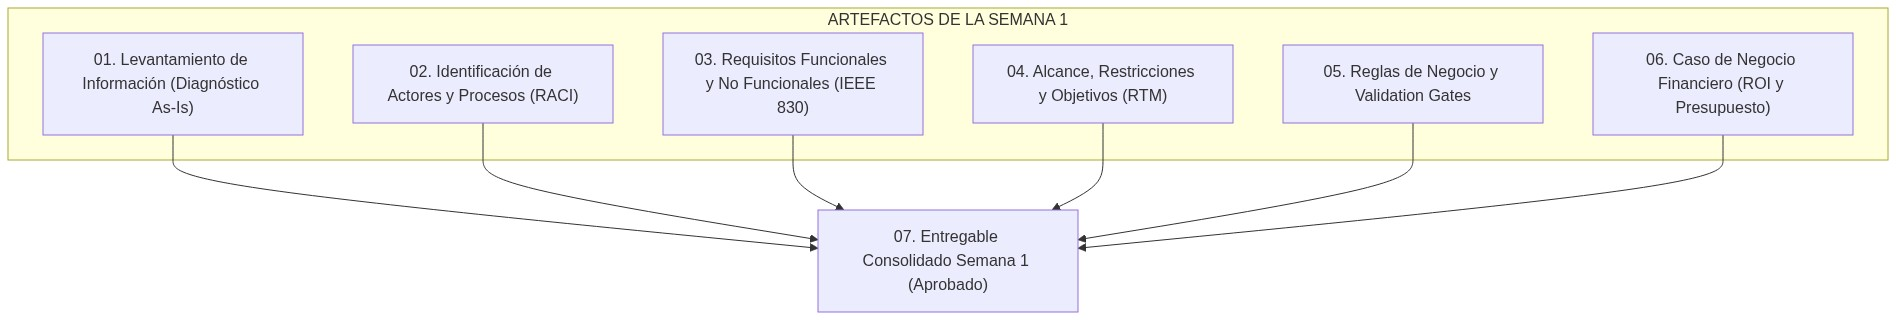
\includegraphics[width=0.85\textwidth,height=4.8cm,keepaspectratio]{images/s1_07_consolidado_s1.png}
    \caption{Mapa de Entregables Consolidados y Flujo de Dependencias de la Semana 1.}
    \label{fig:s1_07_cons}
\end{figure}

\section{Descripción de actividades}

\subsection{Índice de Entregables de la Semana 1 (Estructura EDT)}
\begin{enumerate}[leftmargin=1.5em, itemsep=2.5pt]
    \item \textbf{EDT 1.1 -- Levantamiento de Información del Proceso Actual:} Diagnóstico del flujo manual actual, cuellos de botella y mapeo de formatos SGC (\texttt{UTA-SGC-A-2-1-P7-T1} y \texttt{UTA-SGC-A-2-1-P7-T2}).
    \item \textbf{EDT 1.2 -- Identificación de Actores y Procesos:} Caracterización de los 5 roles (Elaborador, Revisor, Validador, Aprobador, Administrador), matriz de poder/interés y matriz RACI de 10 procesos.
    \item \textbf{EDT 1.3 -- Definición de Requisitos Funcionales y No Funcionales:} 24 requerimientos funcionales y 8 no funcionales formalizados bajo estándar IEEE 830.
    \item \textbf{EDT 1.4 -- Definición del Alcance, Restricciones y Objetivos:} Objetivos SMART, límites del proyecto (In/Out-Scope) y Matriz de Trazabilidad de Requerimientos (RTM).
    \item \textbf{EDT 1.5 -- Reglas de Negocio y Validation Gates:} Formalización lógica de compuertas deterministas, fechas inmutables del servidor, autocompletado y validación de evidencias en MinIO.
    \item \textbf{EDT 1.6 -- Caso de Negocio (Business Case):} Estudio de viabilidad económica, presupuesto de \$630.30 USD, ahorro anual de \$23,700.00 USD, ROI de +3,660.0\% y matriz de mitigación de 5 riesgos.
\end{enumerate}

\subsection{Distribución de Trabajo y Cumplimiento del Equipo}

\begin{table}[htbp]
\centering
\small
\begin{tabularx}{\textwidth}{|>{\hsize=0.7\hsize\bfseries}X|>{\hsize=1.0\hsize}X|>{\hsize=0.45\hsize\centering\arraybackslash}X|>{\hsize=1.2\hsize}X|>{\hsize=0.65\hsize\centering\arraybackslash}X|}
    \hline
    \rowcolor{tableheader}
    Integrante & Rol Principal & Horas & Tareas Culminadas & Estado \\
    \hline
    Steeven Toala & Líder de Proyecto / Arquitecto & 18 h & Scope, Validation Gates, SAD preliminar & \textbf{100\% Completo} \\
    \hline
    Heidy Villavicencio & Analista de Requerimientos / UI-UX & 16 h & Relevamiento As-Is, SRS IEEE 830, RACI & \textbf{100\% Completo} \\
    \hline
    Nixon Hurtado & Desarrollador Backend / DBA & 15 h & Reglas de datos, Modelo ER inicial, MinIO & \textbf{100\% Completo} \\
    \hline
    Andrea Vasquez & Desarrolladora Frontend / QA Tester & 15 h & Pruebas de requerimientos, RTM, RNF & \textbf{100\% Completo} \\
    \hline
    \rowcolor{gray!15}
    \textbf{TOTAL SEMANA 1} & \textbf{Equipo de Desarrollo SIGE} & \textbf{64 h} & \textbf{6 Paquetes de Trabajo EDT} & \textbf{Aprobado} \\
    \hline
\end{tabularx}
\caption{Matriz de Control de Esfuerzo y Desempeño - Semana 1.}
\label{tab:s1_07_esfuerzo}
\end{table}

\subsection{Conclusión y Transición a la Semana 2}
Con la culminación de la Semana 1, el proyecto \textbf{SIGE} cuenta con una base sólida de ingeniería de requerimientos para ingresar a la \textbf{Semana 2: Diseño Rápido y Arquitectura}, donde se generarán los diagramas UML de Casos de Uso, la Clean Architecture en .NET 9, los diagramas de secuencia/clases, el modelo relacional en PostgreSQL 16, los prototipos UI/UX en Figma y la orquestación en Docker Compose.

\vspace{0.3cm}

% =============================================================
% FIRMAS DE RESPONSABILIDAD
% =============================================================
\section{Firmas de Responsabilidad}

\noindent
\renewcommand{\arraystretch}{1.2}
\begin{tabularx}{\textwidth}{|>{\raggedright\arraybackslash}m{2.9cm}|>{\raggedright\arraybackslash}X|>{\centering\arraybackslash}m{4.6cm}|>{\centering\arraybackslash}m{2.3cm}|}
    \hline
    \rowcolor{headerred}
    \textcolor{white}{\textbf{ACCIÓN}} & \textcolor{white}{\textbf{NOMBRE Y CARGO}} & \textcolor{white}{\textbf{FIRMA}} & \textcolor{white}{\textbf{FECHA}} \\
    \hline
    \textbf{Elaborado por:} & Heidy Villavicencio\newline \textit{Analista de Requerimientos / UI-UX} & \parbox[c]{4.4cm}{\centering\vspace{4pt}
\includegraphics[height=1.5cm,width=4.0cm,keepaspectratio]{images/firma_heidi.png}\vspace{4pt}} & 24/08/2026 \\
    \hline
    \textbf{Revisado por:} & Steeven Toala\newline \textit{Líder de Proyecto / Arquitecto Software} & \parbox[c]{4.4cm}{\centering\vspace{10pt}\textbf{\textcolor{gray!80}{\scriptsize [ PENDIENTE DE REVISIÓN ]}}\vspace{10pt}} & \textbf{\textcolor{gray!90}{Pendiente}} \\
    \hline
    \textbf{Aprobado por:} & Ing. Paulo Torres\newline \textit{Docente Tutor - Gestión Proyectos Software} & \parbox[c]{4.4cm}{\centering\vspace{10pt}\textbf{\textcolor{gray!80}{\scriptsize [ PENDIENTE DE APROBACIÓN ]}}\vspace{10pt}} & \textbf{\textcolor{gray!90}{Pendiente}} \\
    \hline
\end{tabularx}

\vspace{0.4cm}

% =============================================================
% CONTROL DE CAMBIOS
% =============================================================
\section{Control de Cambios}

\noindent
\renewcommand{\arraystretch}{1.2}
\begin{tabularx}{\textwidth}{|>{\hsize=0.45\hsize\centering\arraybackslash}X|>{\hsize=1.55\hsize\raggedright\arraybackslash}X|>{\hsize=1.2\hsize\raggedright\arraybackslash}X|>{\hsize=0.8\hsize\centering\arraybackslash}X|}
    \hline
    \rowcolor{gray!20}
    \textbf{Versión} & \textbf{Descripción del cambio} & \textbf{Responsable del cambio} & \textbf{Fecha de aprobación} \\
    \hline
    1.0 & Consolidación final de entregables de la Semana 1 / Pendiente de revisión & Heidy Villavicencio & \textbf{\textcolor{gray!90}{Pendiente de Revisión}} \\
    \hline
\end{tabularx}

\vspace{0.4cm}

\section{Anexos}
\subsection*{Anexo 1: Acta de Validación de Línea Base de Requerimientos}
Se certifica la entrega formal de los 6 documentos técnicos de la Semana 1 para revisión por el docente tutor de la cátedra de Gestión de Proyectos de Software.

\end{document}
